\usetikzlibrary{arrows}
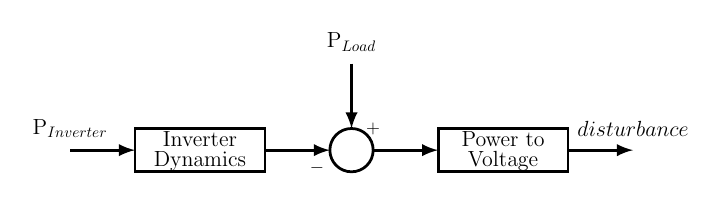
\begin{tikzpicture}[scale=0.55,transform shape]



\node at (-1.5,1.25) {\Large{Inverter}};
\node at (-1.5,0.75) {\Large{Dynamics}};
\draw  [-latex,line width=1pt](-3,1.5) rectangle (0,0.5);
\draw  [-latex,line width=1pt](2,1) ellipse (0.5 and 0.5);
\draw [-latex,line width=1pt](0,1) -- (1.5,1);
\draw [-latex,line width=1pt] (4,1.5) rectangle (7,0.5);
\node at (5.5,1.25) {\Large{Power to}};
\node at (5.5,0.75) {\Large{Voltage}};
\draw [-latex,line width=1pt](2.5,1) -- (4,1);
\draw [-latex,line width=1pt](7,1) -- (8.5,1);
\node at (2.5,1.5) {\large{$+$}};
\node at (1.2,0.6) {\large{$-$}};
\draw [-latex,line width=1pt](2,3) -- (2,1.5);
\node at (2,3.5) {\Large{P$_{Load}$}};
\draw [-latex,line width=1pt](-4.5,1) -- (-3,1);
\node at (-4.5,1.5) {\Large{P$_{Inverter}$}};
\node at (8.5,1.5) {\Large{$disturbance$}};
%\node at (8.3,0.5) {\large{$+$}};
\end{tikzpicture}